% ! TeX root = ../bachelor-thesis.tex

\chapter{Implementazione del prototipo}
\label{ch:Chapter5}

In questo capitolo, si discuterà l’implementazione prima del sistema domotico e
successivamente delle \textit{skill} di Alexa per gli esercizi cognitivi. In
entrambi i casi, saranno anche forniti degli esempi di codice che descriveranno
le interazioni tra le componenti di ciascun sistema.

\section{Implementazione del sistema domotico}
\label{sec:Sezione5.1}

In questa sezione, si illustrerà l’organizzazione del codice per il sistema
domotico e l’implementazione del servizio che permetterà all’utente di
controllare e monitorare i propri dispositivi domotici. Successivamente, sarà
fornito un esempio d'integrazione di un dispositivo domotico a OpenHAB, per il
quale è stata prevista la possibilità di una comunicazione bidirezionale tra
Alexa e OpenHAB.

\subsection{Struttura dei file di configurazione}
\label{subsec:Sezione5.1.1}

Di seguito, viene riportata la struttura standard dei file di configurazione di
OpenHAB (Figura \ref{fig:figure5.1}).

\begin{figure}[!ht]
  \centering
  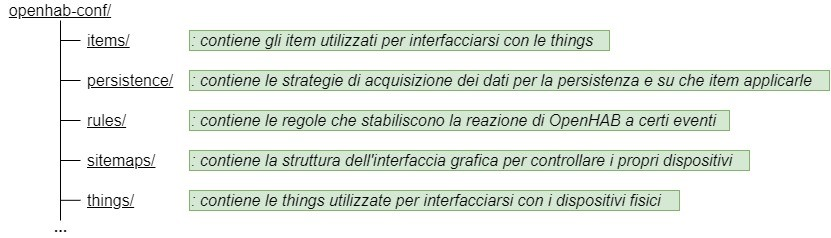
\includegraphics[scale=0.58]{resources/images/implementation/openhab-project-organization.jpg}
  \caption{
    L'organizzazione della directory che contiene i file di configurazione di
    OpenHAB.
  }
  \label{fig:figure5.1}
\end{figure}

I file di configurazione definiscono:

\begin{itemize}
  \item[--] \textit{Things} e \textit{Channels}: i dispositivi fisici connessi
        al sistema e le loro funzionalità;
  \item[--] \textit{Items}: i metodi e i componenti grafici utilizzabili per
        controllare i dispositivi, all’interno dei file di configurazione di
        OpenHAB e dell’interfaccia grafica rispettivamente;
  \item[--] \textit{Sitemaps}: l’organizzazione dei componenti nell’interfaccia
        grafica;
  \item[--] \textit{Rules}: le regole di automazione del sistema domotico,
        ovvero le sue reazioni agli eventi che riceve dai dispositivi che lo
        compongono;
  \item[--] \textit{Persistence}: le regole utilizzate per costruire uno
        storico degli stati degli item specificati.
\end{itemize}

Questi file sono caricati all’avvio della macchina in cui è stato installato
OpenHAB e a ogni loro aggiornamento durante l’esecuzione. Nel caso specifico,
il sistema domotico è stato installato su un \textbf{Raspberry PI}, con sistema
operativo a base \textbf{Linux}.

\subsection{Accesso al sistema domotico}
\label{subsec:Sezione5.1.2}

Per controllare il proprio sistema domotico è possibile accedere alla
\textbf{Dashboard di OpenHAB}, disponibile all’indirizzo IP della macchina su
cui è installato, su una specifica porta.

La dashboard permette di configurare il proprio sistema tramite interfaccia
grafica e d'interagire con le interfacce grafiche realizzate per controllare i
propri dispositivi domotici. In particolare, queste definiscono
l’organizzazione dei componenti grafici che potranno essere usati per
controllare i dispositivi domotici, ma non i componenti grafici stessi
(definiti invece dalle \textit{tipologie di item} usate per rappresentare le
funzionalità di quei dispositivi). I componenti grafici, oltre a controllare un
determinato dispositivo domotico, permettono di accedere allo storico dei suoi
stati in un certo periodo di tempo d’interesse.

Per controllare il sistema domotico, sono state rese disponibili due interfacce
grafiche:
\begin{itemize}
  \item[--] Una \textit{\textbf{sitemap}}: privilegia un’esposizione agevole e
        compatta delle funzionalità del sistema; quest’interfaccia era già stata
        predisposta in un tempo precedente rispetto a questo progetto;
  \item[--] Delle \textit{\textbf{pages}}: privilegiano l’estetica
        dell’interfaccia grafica.
\end{itemize}
Per le \textit{pages}, si è deciso di sfruttare una nuova funzionalità
introdotta nella versione 3.x di OpenHAB: il \textbf{modello semantico}.

Il modello semantico di un certo locale consente di organizzare logicamente i
propri dispositivi domotici, prima in base alla loro posizione nel locale e
successivamente in base alla loro funzionalità. OpenHAB è quindi in grado di:
\begin{itemize}
  \item[--] costruire il modello semantico automaticamente, se il codice
        rispecchia una certa struttura logica;
  \item[--] dal modello semantico, ricavare automaticamente un’interfaccia
        grafica ben strutturata, dalla quale è possibile controllare i propri
        dispositivi domotici.
\end{itemize}
Pertanto, è stato sufficiente riorganizzare la struttura di alcuni file di
configurazione, per ottenere un’interfaccia grafica già impostata, che
consentisse all’utente di controllare e monitorare il proprio sistema
domotico.

\subsection{Esempio d'integrazione con OpenHAB}
\label{subsec:Sezione5.1.3}

Ora sarà illustrato un esempio su come è possibile integrare una lampadina
Philips Hue al sistema domotico.

Innanzitutto, è necessario installare sul proprio sistema domotico un
\textit{add-on}, chiamato \textbf{Philips Hue Binding} \cite{BINDING_PH}.
Questo definirà alcune \textit{tipologie di thing}, che hanno \textit{channels}
preconfigurati per comunicare con dispositivi fisici della Philips Hue.

A questo punto è possibile iniziare a integrare i propri dispositivi domotici,
dichiarando le \textit{\textbf{things}} del sistema in un file
\textit{.things}.

\begin{figure}[!ht]
  \centering
  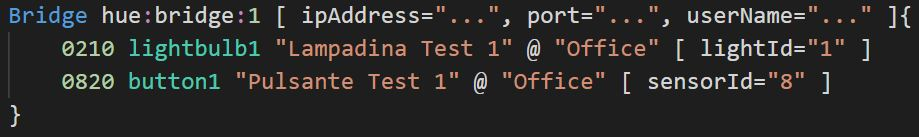
\includegraphics[scale=0.65]{resources/images/implementation/code/thing-code-example.jpg}
  \caption{
    Un esempio di file di configurazione per le \textit{thing}: in questo caso
    è stato dichiarato un bridge con due dispositivi connessi, una lampadina e
    un pulsante.
  }
  \label{fig:figure5.2}
\end{figure}

Nell’esempio (Figura \ref{fig:figure5.2}), viene integrato un \textbf{bridge
Hue} a cui sono collegati una \textbf{lampadina} e un \textbf{pulsante} della
Philips Hue. Queste sono le \textit{things} vere e proprie e sono
contraddistinte da due proprietà principali:
\begin{itemize}
  \item[--] Il \textit{\textbf{tipo di thing}}, che dichiara i \textit{channel}
        disponibili a quella \textit{thing}, ovvero le funzionalità del
        dispositivo. In questo caso, sono forniti dal \textit{binding} del
        produttore specifico (nell’esempio: \textit{0210} e \textit{0820});
  \item[--] Il \textit{\textbf{nome della thing}}, che serve per riconoscerla
        all’interno dei file di configurazione di OpenHAB (nell’esempio:
        \textit{lightbulb1} e \textit{button1}).
\end{itemize}

Una volta integrati i dispositivi domotici al sistema OpenHAB, bisogna definire
come sarà possibile controllarli nei file di configurazione e nell’interfaccia
grafica, dichiarando gli \textit{\textbf{items}} del sistema in un file
\textit{.items}.

\begin{figure}[!ht]
  \centering
  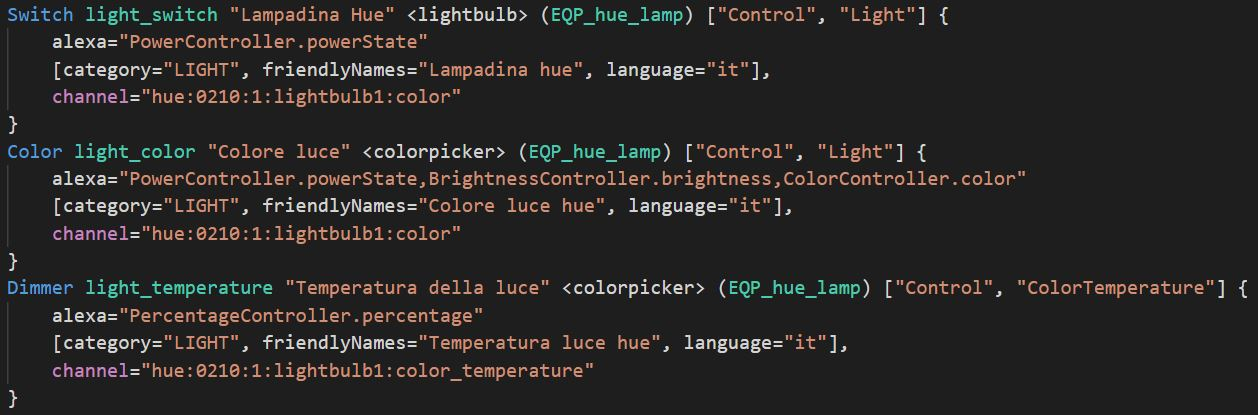
\includegraphics[scale=0.48]{resources/images/implementation/code/items-code-example.jpg}
  \caption{
    Un esempio di file di configurazione per gli \textit{items}: in questo caso
    sono state esposte le funzionalità di una lampadina Hue, che comprendono
    l'accensione, il colore e la temperatura del colore.
  }
  \label{fig:figure5.3}
\end{figure}

Nell’esempio (Figura \ref{fig:figure5.3}) sono stati creati tre \textit{items}
per la lampadina integrata precedentemente: uno \textbf{Switch} per accendere e
spegnere la lampadina, un \textbf{Color} per impostarne il colore e un
\textbf{Dimmer} per regolarne la temperatura del colore. I punti focali della
sintassi di un \textit{item} sono:
\begin{itemize}
  \item[--] Il \textit{\textbf{tipo di item}}, che definisce come sarà
        possibile interagire con le funzionalità che controlla. I \textit{tipi
          di item} sono standard e ognuno fornisce gli stati che può assumere
        l’\textit{item} e i comandi che può ricevere. Ad esempio, uno Switch
        può essere acceso (\textit{ON}) o spento (\textit{OFF});
  \item[--] Il \textit{\textbf{nome dell’item}}, che serve per riconoscerlo
        all’interno dei file di configurazione di OpenHAB (nell’esempio
        \textit{light\_switch}, \textit{light\_color} e
        \textit{light\_temperature});
  \item[--] Il \textit{\textbf{channel associato}}, che definisce le
        funzionalità che l’\textit{item} controlla e il ponte tra
        \textit{item} e \textit{thing}. In questo caso, la sintassi usata per
        identificare un \textit{channel} è definita dal \textit{binding} a cui
        appartiene, ovvero Philips Hue Binding (nell’esempio:
        \textit{channel=”hue:0210:1:lightbulb1:color”} permette di controllare
        il colore e lo stato di accensione della \textit{thing}
        \textit{lightbulb1}).
  \item[--] L’\textit{\textbf{interfaccia di Alexa implementata}}, che serve
        per configurare la \textbf{skill di OpenHAB} per Alexa. In particolare,
        indica con quali comandi vocali si potrà controllare
        quell’\textit{item} attraverso un dispositivo Alexa (nell’esempio:
        \textit{alexa= ”PowerController.PowerState” […]}).
\end{itemize}

A questo punto è già possibile controllare i propri dispositivi domotici
tramite Alexa e, assumendo che la sintassi rispetti le regole del modello
semantico di OpenHAB, anche attraverso un'interfaccia grafica, generata
automaticamente, su OpenHAB.

L’ultima cosa che rimane da fare, è quella di notificare l’utente degli eventi
rilevati da OpenHAB. A questo proposito, sarà necessario installare un altro
\textit{add-on} sul proprio sistema domotico: \textbf{Amazon Echo Control
Binding}. Questo \textit{binding} permetterà d'integrare un dispositivo Alexa a
OpenHAB, con un metodo analogo a quello utilizzato per la lampadina Hue.
Dunque, sarà possibile controllarlo attraverso una regola di automazione,
definendo una \textit{\textbf{rule}} in un file \textit{.rules}.

\begin{figure}[!ht]
  \centering
  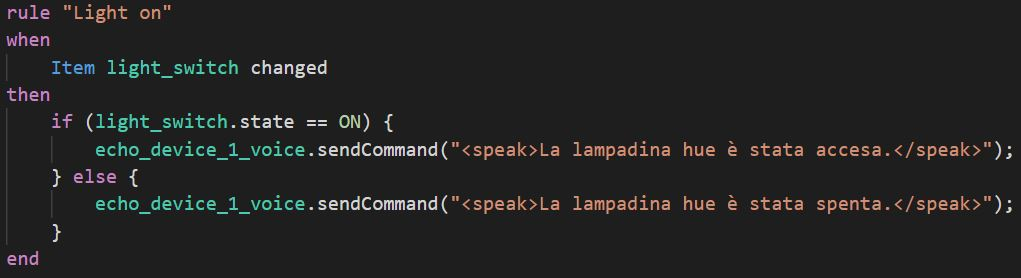
\includegraphics[scale=0.59]{resources/images/implementation/code/rule-code-example.jpg}
  \caption{
    Un esempio di file di configurazione per le \textit{rules}: in questo caso
    è stato definito un \textit{handler} che reagisce ai cambiamenti di stato
    della lampadina Hue, comunicandoli all'utente tramite un dispositivo Alexa.
  }
  \label{fig:figure5.4}
\end{figure}

Nell’esempio (Figura \ref{fig:figure5.4}), viene definita una regola che
risponde ai cambiamenti dello stato di accensione della lampadina Hue (ovvero
se è stata accesa o spenta), controllando un dispositivo Alexa Echo e quindi
comunicando all’utente il nuovo stato della lampadina.

\section{Implementazione delle skill}
\label{sec:Sezione5.2}

In questa sezione, si illustrerà l’organizzazione del codice per il progetto
del servizio che espone gli esercizi cognitivi e l’implementazione
dell’interazione tra l’utente e tale servizio. Infine, saranno presentati
alcuni estratti di codice che aiutino a visualizzare nel concreto le componenti
del sistema e le loro interazioni.

Per l’implementazione è stato utilizzato il linguaggio di programmazione
\textbf{TypeScript} \cite{TYPESCRIPT}, che è un’estensione tipizzata di
\textbf{JavaScript}. Il servizio è stato costruito sul framework
\textbf{node.js} \cite{NODE.JS}, il cui scopo è gestire applicazioni di rete
scalabili, e in particolare sul framework \textbf{Express} \cite{EXPRESS},
utilizzato per costruire applicazioni web.

\subsection{Struttura dell'applicazione}
\label{subsec:Sezione5.2.1}

Di seguito, viene riportata la struttura organizzativa utilizzata nella
directory del progetto sugli esercizi cognitivi (Figura \ref{fig:figure5.5}).
Sono quindi evidenziate, le componenti principali del progetto e la loro
funzione.

\begin{figure}[!ht]
  \centering
  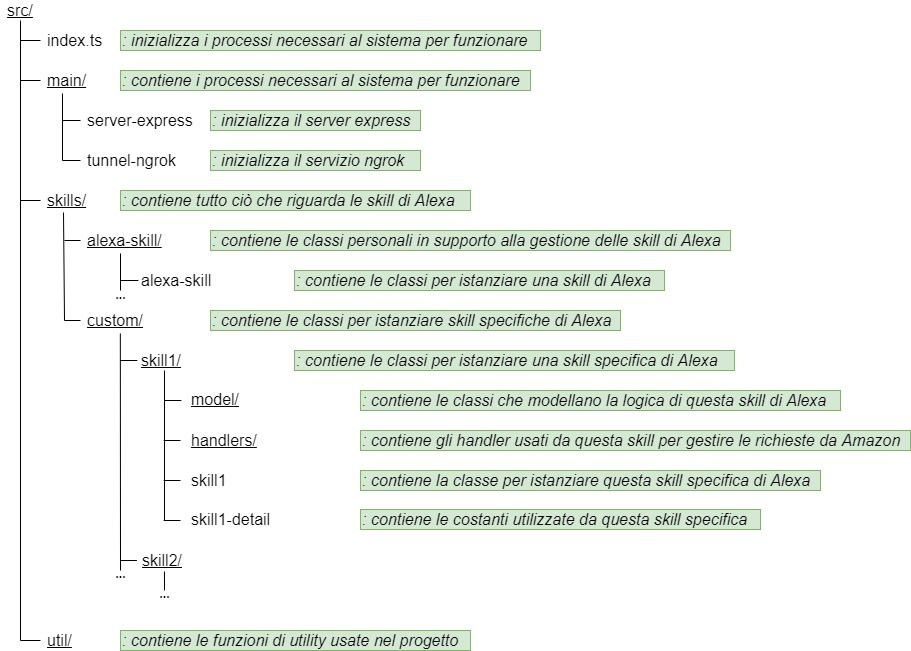
\includegraphics[scale=0.58]{resources/images/implementation/alexa-project-organization.jpg}
  \caption{
    L'organizzazione della directory che contiene l'applicazione che gestisce
    il servizio per le \textit{skill} cognitive.
  }
  \label{fig:figure5.5}
\end{figure}

\subsection{Funzionamento dell'applicazione}
\label{subsec:Sezione5.2.2}

All’avvio, l’applicazione crea il \textbf{server Express} utilizzato per
accedere al servizio. Questo potrà ricevere le \textit{richieste http}
dell’utente, delegandone la gestione ad alcuni \textit{handler}, selezionati in
base al \textit{percorso} specificato dall’utente. Successivamente, viene
verificata l’esistenza di un \textbf{tunnel ngrok} verso la porta del
\textit{server Express}: se non è presente, viene avviato un nuovo processo,
che eseguirà \textit{ngrok} in modo indipendente dall’applicazione. Il processo
\textit{ngrok} dovrà rimanere attivo anche dopo la chiusura dell’applicazione,
così non sarà riavviato insieme all’applicazione. Infatti, per inizializzare
l’applicazione, è stato utilizzato il processo \textit{Nodemon} per Node.js,
che, una volta avviato, rileva ogni aggiornamento sulla directory indicatagli,
reagendo con un riavvio automatico dell’applicazione, quindi applicando le
modifiche eseguite sul codice.

All’inizializzazione del \textit{server Express}, vengono anche creati i
gestori delle richieste http. Questi consistono nelle vere e proprie
\textbf{skills di Alexa}. Ogni \textit{skill} viene associata al \textit{server
Express} su uno specifico percorso, tramite un \textbf{Express Adapter}, che si
occuperà di validare le richieste http in entrata, controllando che
effettivamente provengano da Amazon Alexa.

Una \textit{skill} avrà il compito di gestire tutte le richieste http sul
percorso assegnatole. Più in dettaglio, riceverà tutte le \textit{intenzioni}
dell’utente che le competono e le smisterà verso gli opportuni \textbf{intent
handlers}. Ogni \textit{intent handler} gestirà una specifica intenzione
dell’utente, interagendo con il \textbf{modello della skill}, che contiene le
classi che descrivono la logica del gioco cognitivo implementato. Al termine
dell’esecuzione, un \textit{intent handler} produrrà un’opportuna risposta, che
sarà comunicata mediante il dispositivo Alexa.

I progressi di un relativo giocatore durante il gioco, vengono memorizzati
sulle variabili di sessione della \textit{skill}, chiamate
\textit{\textbf{session attributes}}. La sessione di una certa \textit{skill} è
relativa all’interazione con uno specifico utente e viene creata all’apertura
della \textit{skill}, permanendo fino alla sua chiusura. Specificamente, è
mantenuta all’interno dei messaggi scambiati tra l’utente e il servizio.

Di seguito, viene riportato uno schema che riassume i componenti descritti
precedentemente (Figura \ref{fig:figure5.6}).
\begin{figure}[!ht]
  \centering
  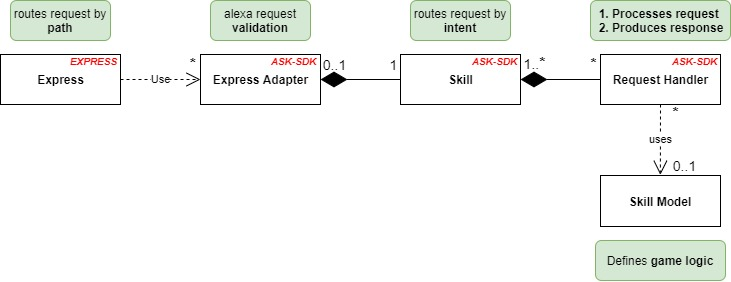
\includegraphics[scale=0.6]{resources/images/implementation/project-class-diagram.jpg}
  \caption{
    Schema che descrive i componenti principali dell'applicazione in base alla
    loro funzione.
  }
  \label{fig:figure5.6}
\end{figure}

Al termine dell’avvio, il \textit{server Express} mostrerà le caratteristiche
del servizio, come mostrato in Figura \ref{fig:figure5.7} (da notare che il
caricamento del server impiega molto tempo quando il servizio \textit{ngrok}
non è già in esecuzione).

Siccome l’indirizzo pubblico del proprio servizio cambia a ogni esecuzione di
\textit{ngrok} (nella licenza gratuita), è necessario ricordarsi di mantenere
aggiornati gli \textit{\textbf{endpoint}} utilizzati dalle \textit{skill}. Gli
\textit{endpoint} sono modificabili dal modello di dialogo delle
\textit{skill}, accessibile dall’\textit{Alexa Skills Kit} dell’\textit{Amazon
Developer Console}. Nella figura, questi endpoint hanno gli indirizzi URL
mostrati nella sezione \textit{LOADED SKILLS}.

\begin{figure}[!ht]
  \centering
  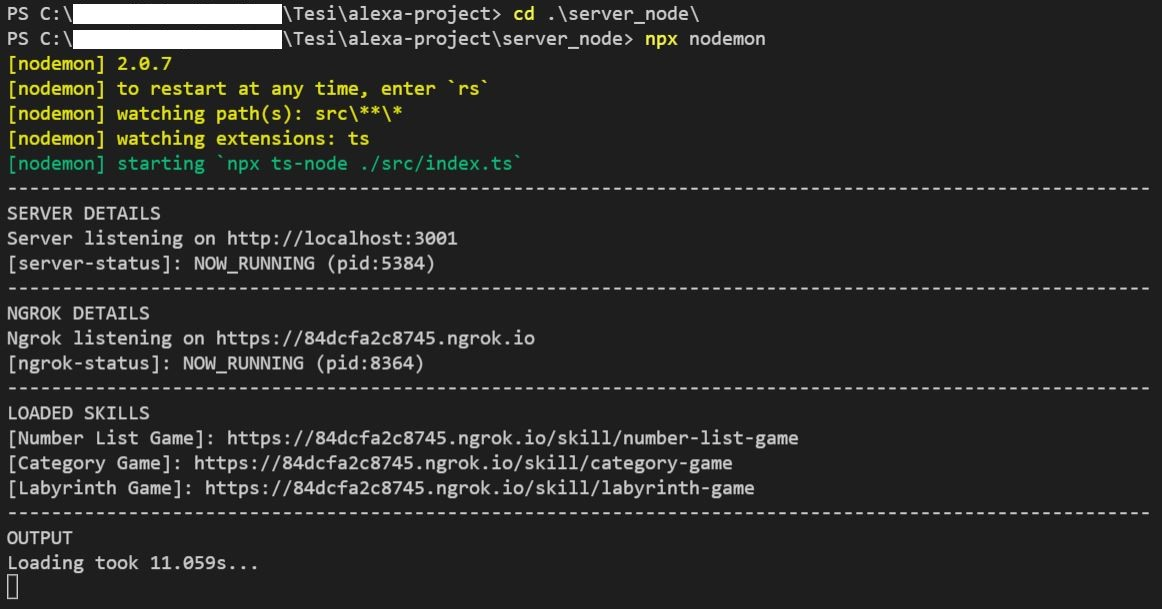
\includegraphics[scale=0.5]{resources/images/implementation/code/express-server-starting-capture.jpg}
  \caption{
    Output del \textit{server Express} dopo la sua inizializzazione. Di
    particolare importanza è la sezione \textit{LOADED SKILLS}.
  }
  \label{fig:figure5.7}
\end{figure}

Una volta finita la configurazione, il servizio è pronto per essere acceduto da
un qualsiasi dispositivo Alexa, che sia associato a un account Amazon in cui
sono installate le \textit{skill}. Siccome non è ancora stato eseguito il
deployment delle \textit{skill}, queste saranno accessibili solo dall’account
che le sta sviluppando.

\subsection{Esempio d'implementazione di una skill}
\label{subsec:Sezione5.2.3}

Ora sarà illustrato un esempio su come è possibile implementare una
\textit{skill}, raggiungibile attraverso un server realizzato con
\textit{Express}.

Inizialmente, è necessario configurare il \textbf{server Express} (Figura
\ref{fig:figure5.8}). Ciò significa creare le \textbf{skills} che dovrà gestire
e mapparle a un determinato percorso nel server. Siccome, su quei percorsi si
vuole accettare solo richieste provenienti da Alexa, viene utilizzato un
\textbf{Express Adapter}, il cui scopo è modificare gli \textit{handler} di una
\textit{skill}, in modo che eseguano una verifica sulla sorgente della
richiesta, preliminarmente alla sua gestione. Il \textit{server Express} si
occuperà di smistare le richieste in entrata in base al percorso da loro
indicato, delegandole alla \textit{skill} opportuna.

\begin{figure}[!ht]
  \centering
  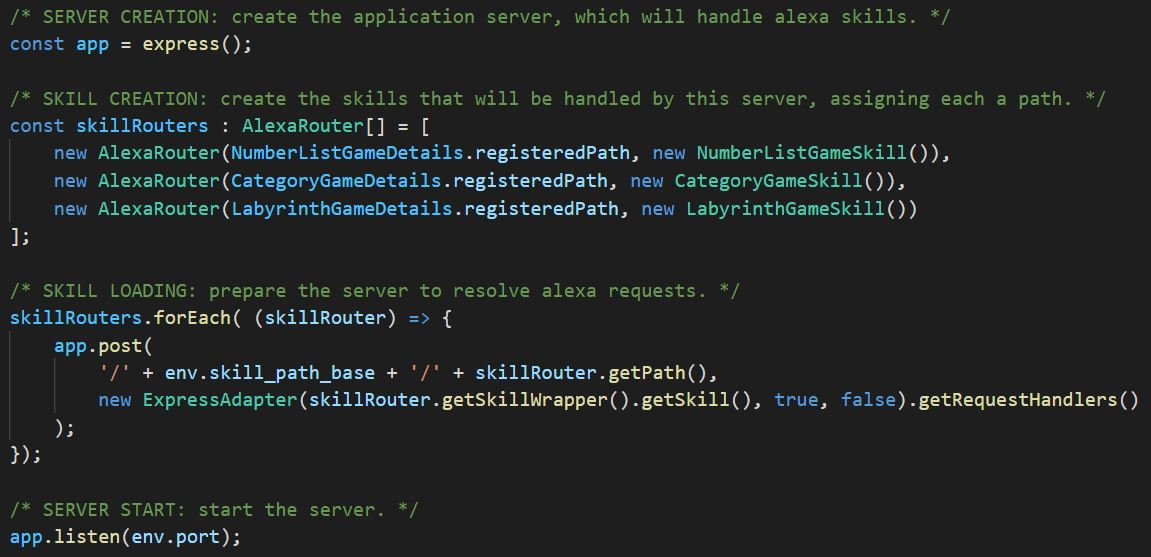
\includegraphics[scale=0.52]{resources/images/implementation/code/server-start-code-example.jpg}
  \caption{
    Inizializzazione del \textit{server Express}. Include la creazione delle
    \textit{skill} e la loro mappatura sul server.
  }
  \label{fig:figure5.8}
\end{figure}

\begin{figure}[!ht]
  \centering
  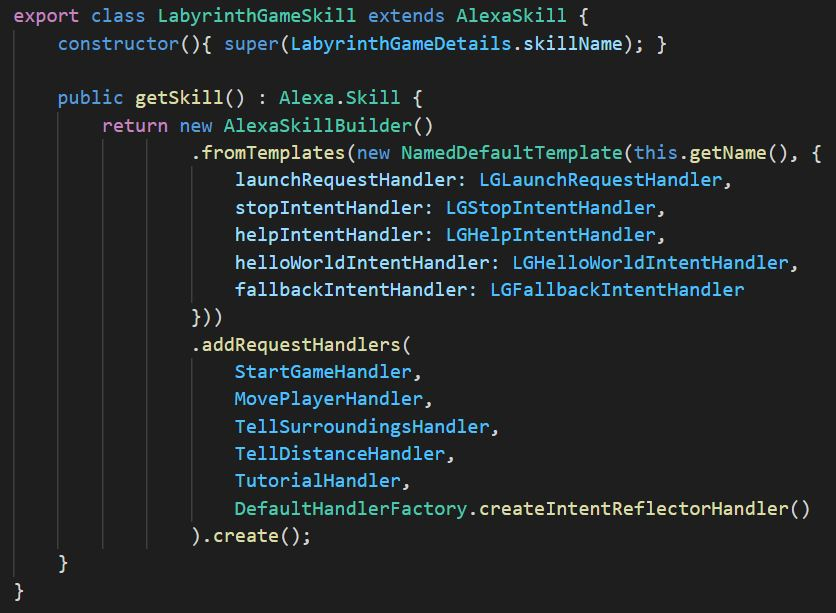
\includegraphics[scale=0.52]{resources/images/implementation/code/skill-code-example.jpg}
  \caption{
    Inizializzazione di una \textit{skill}. Qui sono inizializzati tutti
    gli \textit{intent handler} utilizzati dalla \textit{skill}.
  }
  \label{fig:figure5.9}
\end{figure}

La creazione di una \textit{skill} (Figura \ref{fig:figure5.9}) avviene
attraverso uno \textbf{Skill Builder}, che ne determina gli \textit{handler}.
Lo \textit{Skill Builder} utilizzato è un’estensione di quello fornito dalla
libreria \textbf{ASK-SDK} e distingue gli handler in due categorie:
\begin{itemize}
  \item[--] Gli \textit{handler standard}, che sono molto simili tra le varie
        \textit{skill}, quindi si prestano bene a essere raggruppati in un
        \textbf{template}, applicabile su \textit{skill} diverse. Ad esempio,
        sono considerati standard gli \textit{handler} indicati da Amazon come
        necessari al deployment di una \textit{skill};
  \item[--] Gli \textit{handler custom} che caratterizzano una specifica
        \textit{skill}, in base alle funzionalità che offre.
\end{itemize}
Ogni \textit{skill} si occuperà di gestire le richieste su di uno specifico
percorso del server in base all’intenzione espressa dall’utente, delegandole
all’\textit{handler} opportuno.

Gli \textit{handler di una skill} sono caratterizzati da due metodi principali
(Figura \ref{fig:figure5.10}). Una funzione, chiamata
\textit{\textbf{canHandle}}, permette alla \textit{skill} di verificare se
l’\textit{handler} può gestire una certa richiesta. Una volta verificato ciò,
può essere applicata la seconda funzione, chiamata \textit{\textbf{handle}},
che gestisce la richiesta. Gli \textit{handler} interagiranno con il modello
della \textit{skill}, controllando il progresso nel gioco, la cui logica è
definita nel modello stesso. Il progresso nel gioco sarà memorizzato nei
parametri della sessione attiva tra l’utente e la \textit{skill} specifica.

\begin{figure}[!ht]
  \centering
  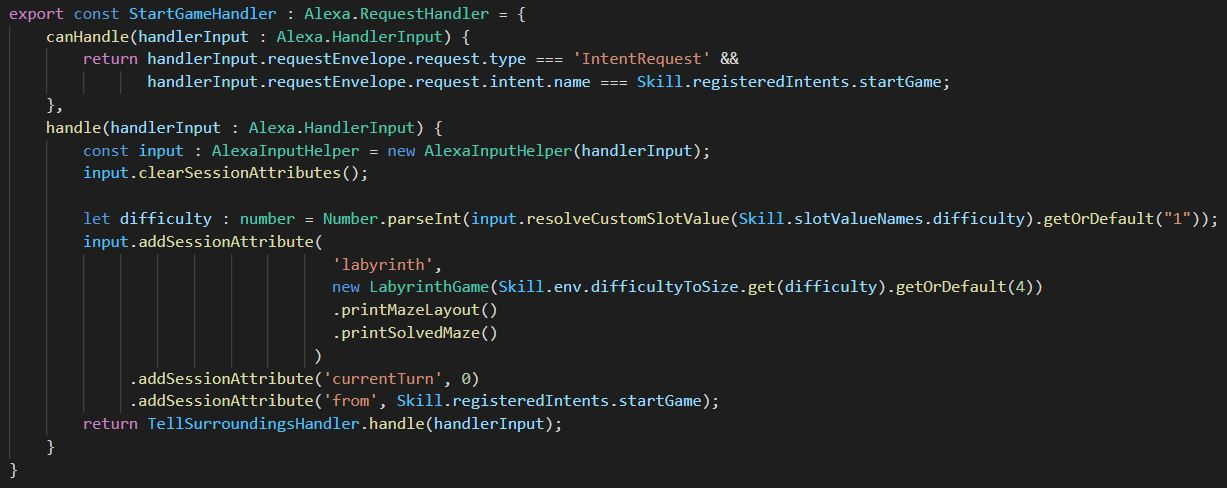
\includegraphics[scale=0.49]{resources/images/implementation/code/skill-handler-code-example.jpg}
  \caption{
    Esempio d'implementazione di un \textit{intent handler}. Si notano i
    caratteristici metodi di un intent handler e l'interazione con il modello
    della skill (ovvero la classe \textit{LabyrinthGame}).
  }
  \label{fig:figure5.10}
\end{figure}

Normalmente, un \textit{handler} produce anche una risposta, che sarà
comunicata dal dispositivo Alexa. Nell’esempio però, la generazione della
risposta è delegata a un altro \textit{handler} della \textit{skill}.
